\documentclass[12pt]{article}
\usepackage[a4paper,bindingoffset=0.2in,
            left=1in,right=1in,top=1in,bottom=1in,
            footskip=.25in]{geometry}
\usepackage{graphicx}
\usepackage{parskip}
\usepackage{titling}
\usepackage[utf8]{inputenc}
\graphicspath{ {images/} }
\begin{document}
\begin{titlepage}
    \begin{center}
        \vspace*{1cm}
        
        \Huge
        \textbf{Technical Specification}
        
        \vspace{0.5cm}
        \LARGE
        SDP Group 15-H
        
        \vspace{1.5cm}
        \normalsize
        Julijonas Kikutis\\ 
		Patrick Green\\
		Aseem Narang\\
		Ankit Sonkar\\
		David McArthur\\
		Emilia Bogdanova
        
        \vfill
        
        
        \vspace{0.8cm}
        
        \begin{figure}
    	\vspace*{-3em}
    	\centering
    	
\includegraphics[scale=.30]{logo.png}
		\end{figure}
        
        \Large
        University of Edinburgh\\
        
    \end{center}
\end{titlepage}

\tableofcontents

\newpage

\section{System Architecture}

Venus has gone through several stages of changes. The earliest prototype had four regular wheels as seen in Figure \ref{fig:robot0}. This made us realise that we have to keep in mind the space
constraints when building the base as we need to accommodate not only the motors
for the wheels but also the kicking and grabbing mechanism. 
\\The next, more sophisticated design, was a robot with four powerful kickers that used elastics as seen in Figure \ref{fig:robot3}. The idea was to stretch elastics for all four kickers using the star shape element on top of the robot as seen in the picture and then release. This gave a lot of energy to the ball. However, this design had a disadvantage because the robot was not able to kick the ball for varying distances, which was an essential requirement for the first milestone. Moreover, the dimensions of the robot were exceeding the maximum size limits and the speed of the ball was exceeding the one allowed in the game rules. 

\begin{figure}[h]
	\centering
	\begin{minipage}[b]{.48\textwidth}
        \centering
		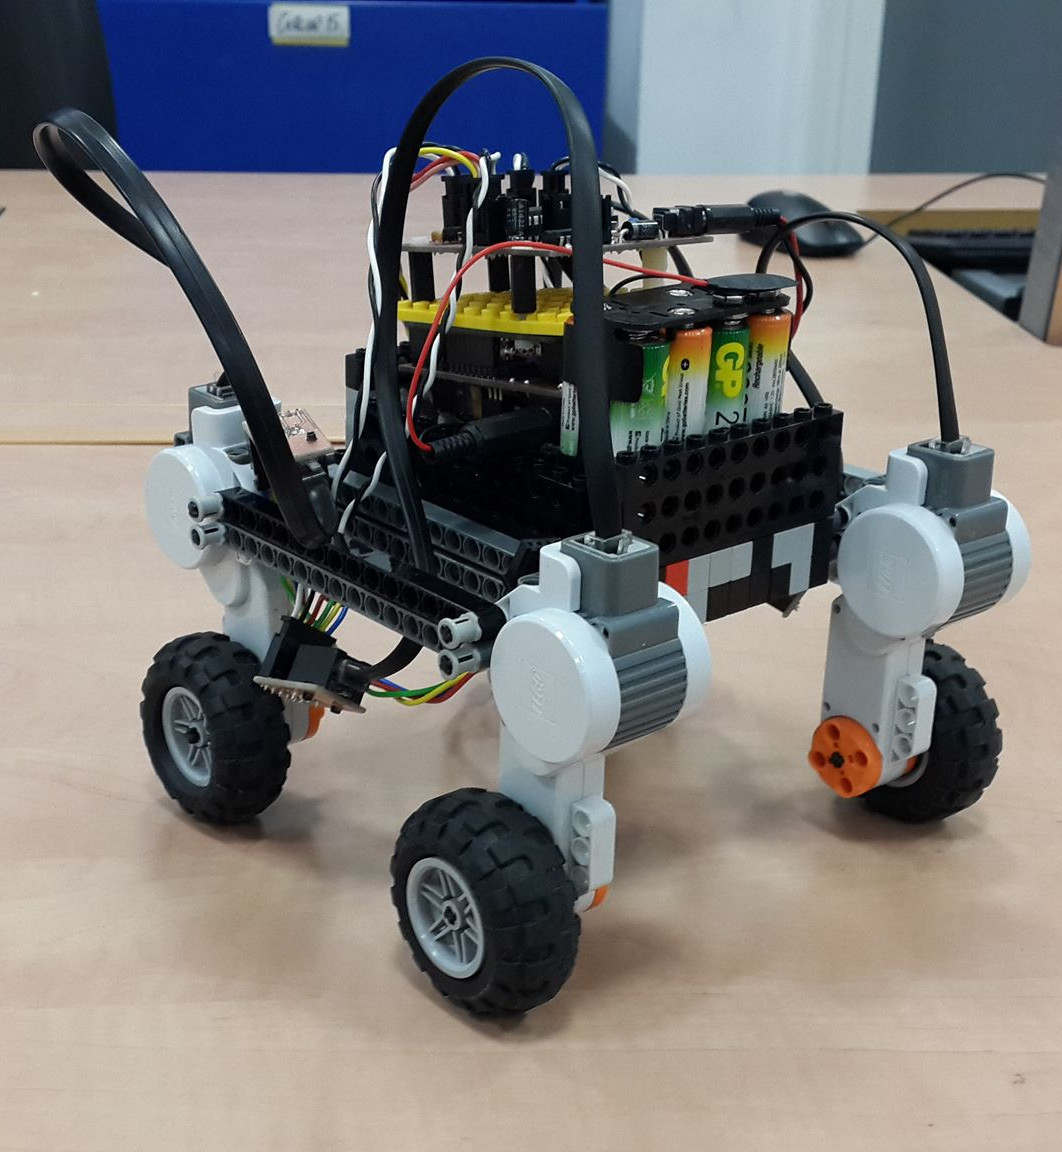
\includegraphics[scale=.18]{robot0.jpg}
		\caption{The first prototype}
		\label{fig:robot0}
	\end{minipage}
	~
	\begin{minipage}[b]{.48\textwidth}
        \centering
		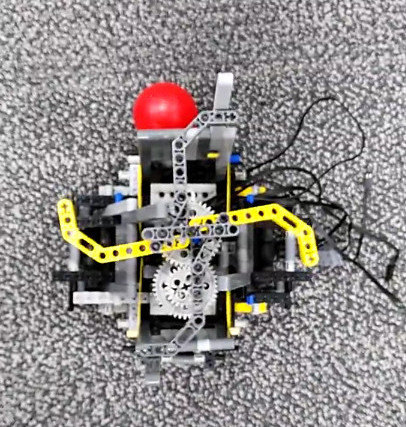
\includegraphics[scale=.65]{robot3.jpg}
		\caption{The robot with four kickers}
		\label{fig:robot3}
	\end{minipage}
\end{figure}

Taking all the disadvantages of previous designs into account we came up with a new design as seen in Figures \ref{fig:open} and \ref{fig:closed}. Advantage of this design is that it is simple and at the same time the robot can still move fast enough to play football and the power of the kicks can be precisely controlled. 

The grabbing mechanism for this design went through two iterations of development.
The first grabber we developed was falling down on the ball in order to catch it, thus was deemed not suitable because it obstructed the ball more than it was allowed by the football game rules. Venus also had difficulties at placing the ball in front of the kicker at initial kicking position, because the grabber pushed it
too far inside the kicker. Thus, the grabber was replaced by the newer design depicted in Figure \ref{fig:open} which has two symmetrical grabbers that interlock when the robot is moving to conserve space and are able to reach a more distant ball.

\begin{figure}[ht]
	\centering
	\begin{minipage}[b]{.48\textwidth}
        \centering
		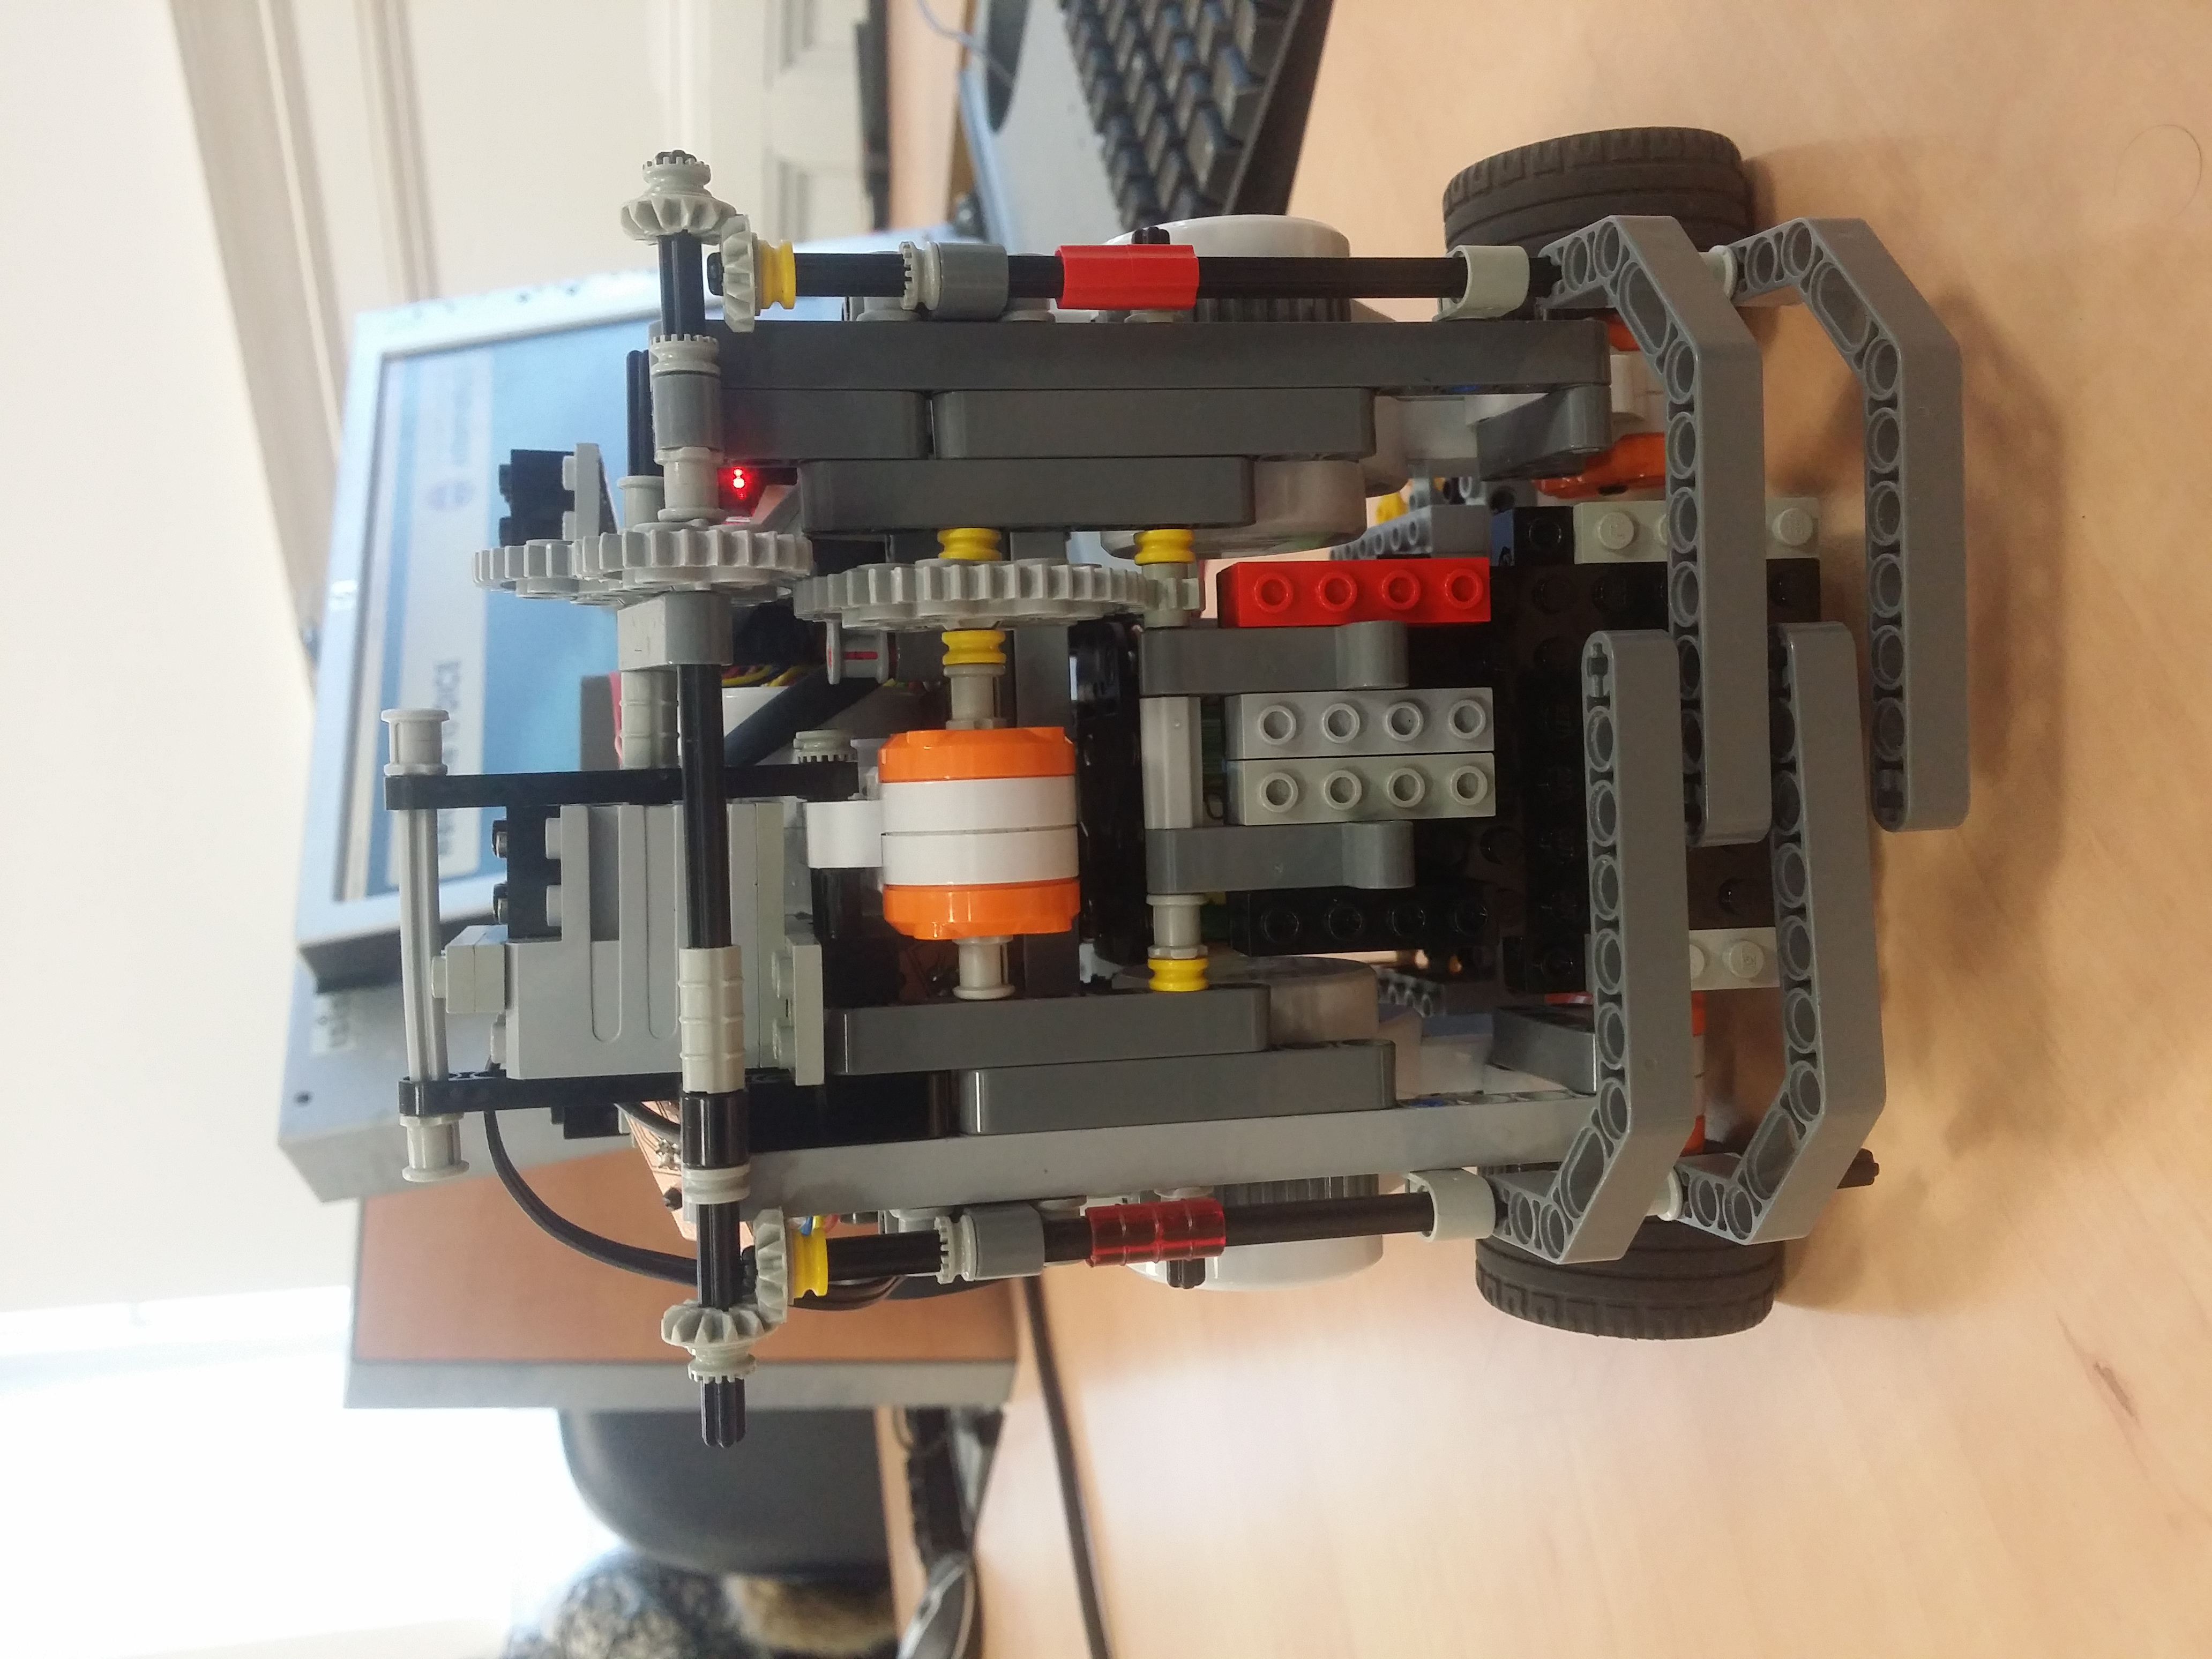
\includegraphics[scale=0.065, angle=-90]{closed_front.jpg}
		\caption{With grabber in closed position}
		\label{fig:closed}
	\end{minipage}
	~
	\begin{minipage}[b]{.48\textwidth}
        \centering
		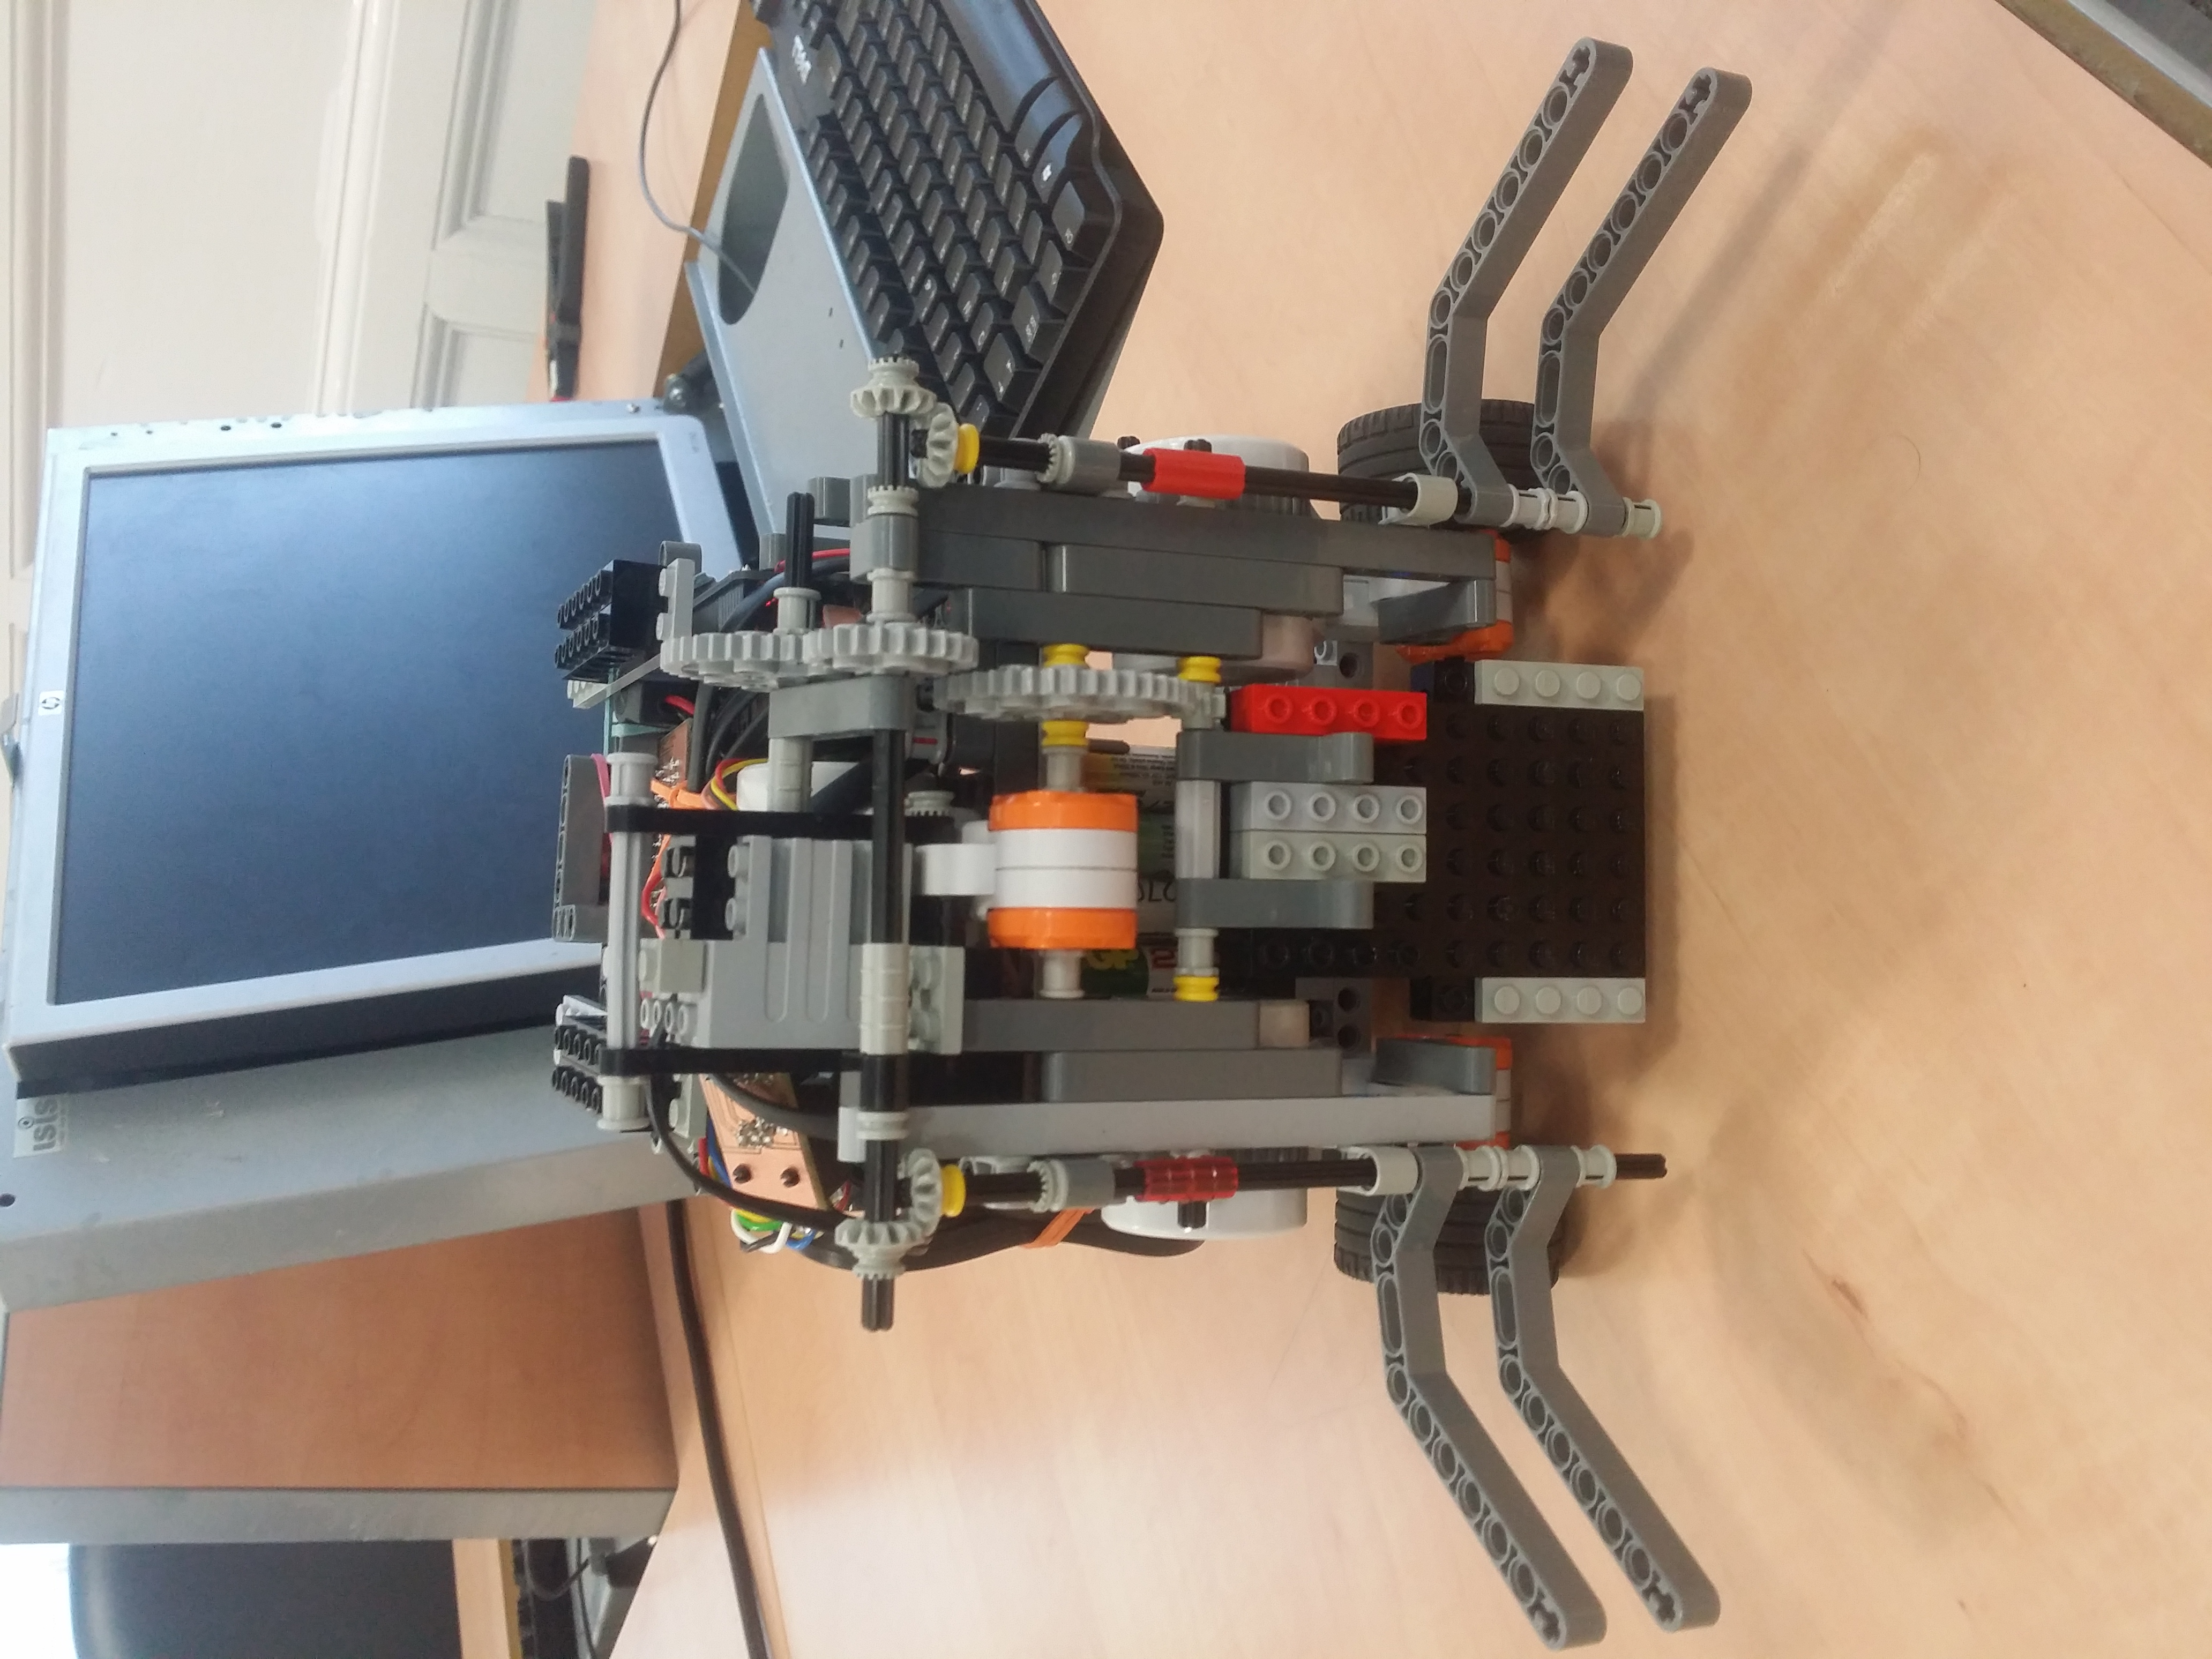
\includegraphics[scale=0.065, angle=-90]{grab_open.jpg}
		\caption{With grabber in open position}
		\label{fig:open}
	\end{minipage}
\end{figure}

After playing the first friendly, we have realized that Venus isn't fast enough comparing to other robots. We decided to start the design from scratch again. Our latest design has four holonomic wheels, which allow Venus to move fast and also in different directions (Figure FIGURE). We had also refused of using any kickers, because none of the kickers we thought of, could fit with four NXT motors. Venus kicks using its grabber and spinning action. The design of the grabber hasn't changed much from the previous time. 

When we were satisfied with the look of Venus, we also made all cables look neat using elastics. We also ensured that we can still access the battery pack and Arduino board if needed as seen in Figure \ref{fig:battery}.

\begin{figure}
	\centering
	\begin{minipage}[b]{.48\textwidth}
        \centering
		\includegraphics[scale=.065]{battery1.jpg}
		\caption{Battery pack easily accessible}
		\label{fig:battery}
	\end{minipage}
	~
	\begin{minipage}[b]{.48\textwidth}
        \centering
		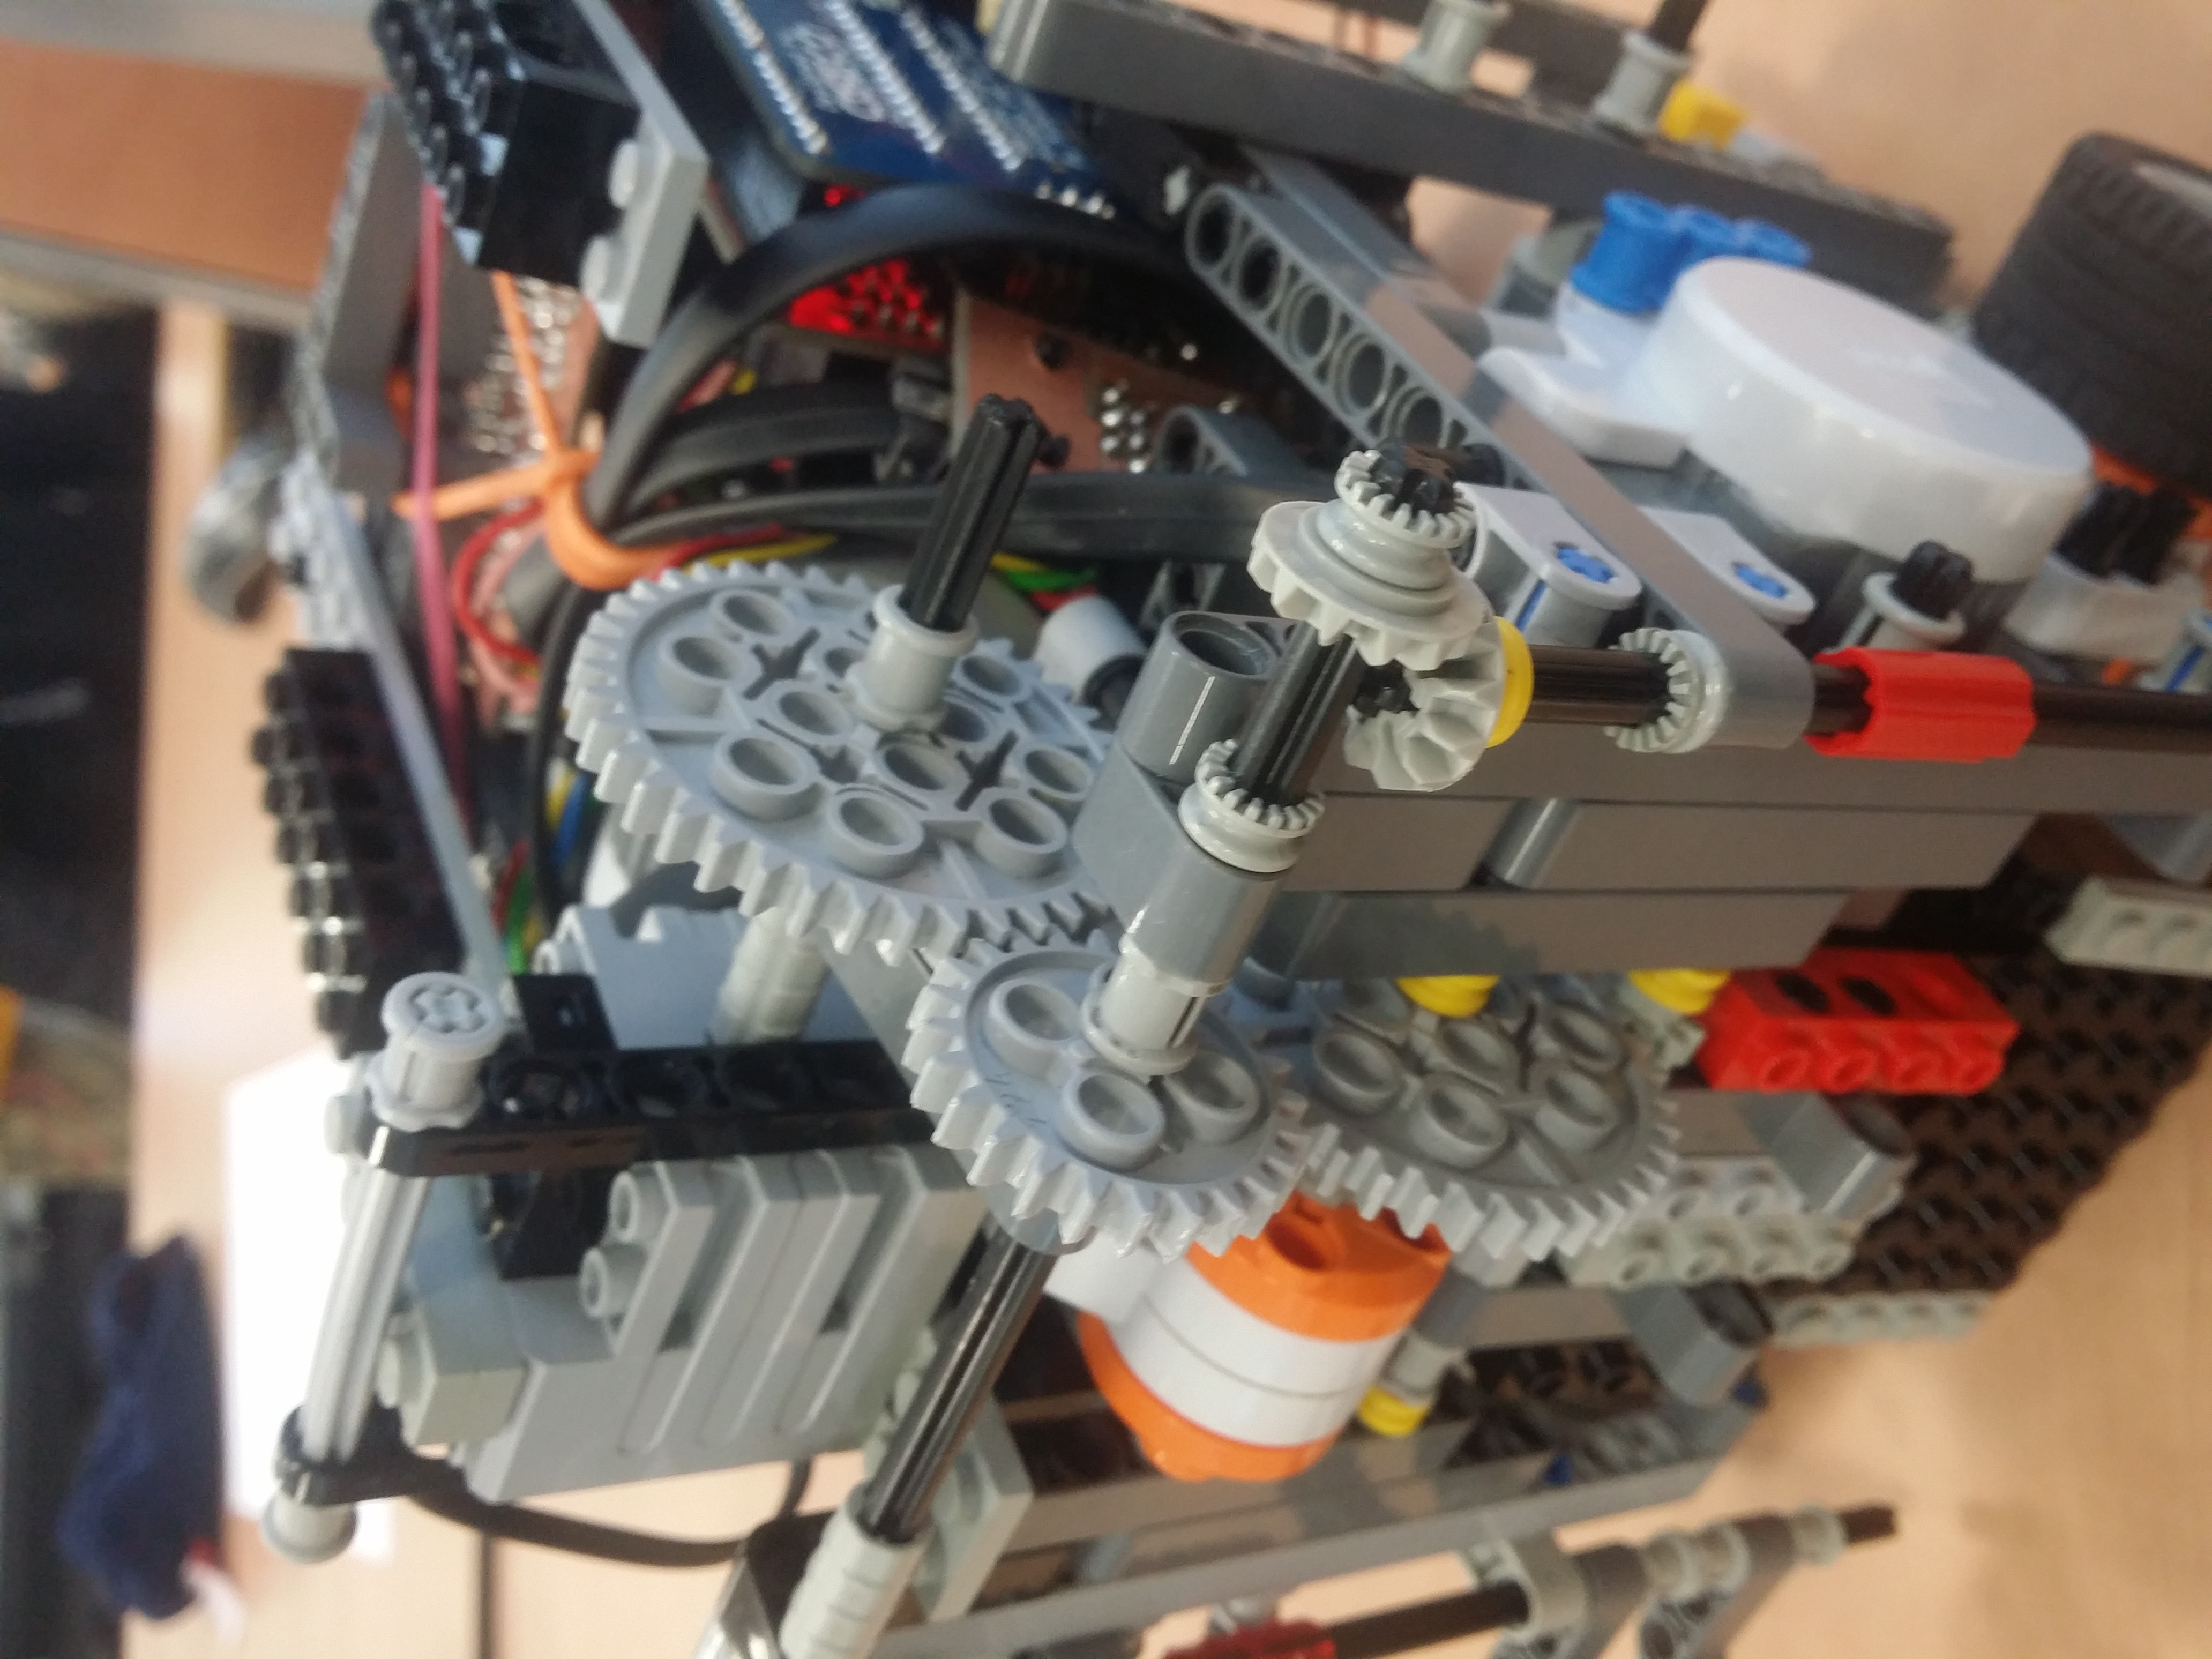
\includegraphics[scale=.065,angle=-90]{gears.jpg}
		\caption{Gears for the grabber}
		\label{fig:gears}
	\end{minipage}
	
\end{figure}


\section{Hardware components}

\subsection{Wheels}
Could you be more descriptive? i.e. why you decided to build it like that ? Why mixture of wheel types ? How the robot can turn? what kind of problems you were trying to omit ? It is a far to short and vague description.  Since your robot has four holonomic wheels now, could you describe why it is a four-wheeled robot now? What is the main feature, advantage of the holonomic property? What is exactly this property.  What are NXT motors ? how they work?


The current design has four holonomic wheels, which allows Venus to move in any direction. All wheels are powered by NXT motors.
\subsection{Kicker}
Even though the idea of the kicker that uses elastics was appealing as this made
the kick more powerful, it was almost impossible to predict the distance the
ball will travel. Because of that the newer design had a
kicker that was powered by an NXT motor with gears. The kicker operated by going backwards inside the robot from the starting low position as seen in Figures \ref{fig:kicker}-\ref{fig:kicker_back} and then kicked
forwards and touched the ball.
\begin{figure}[ht]
	\centering
	\begin{minipage}[b]{.3\textwidth}
        \centering
		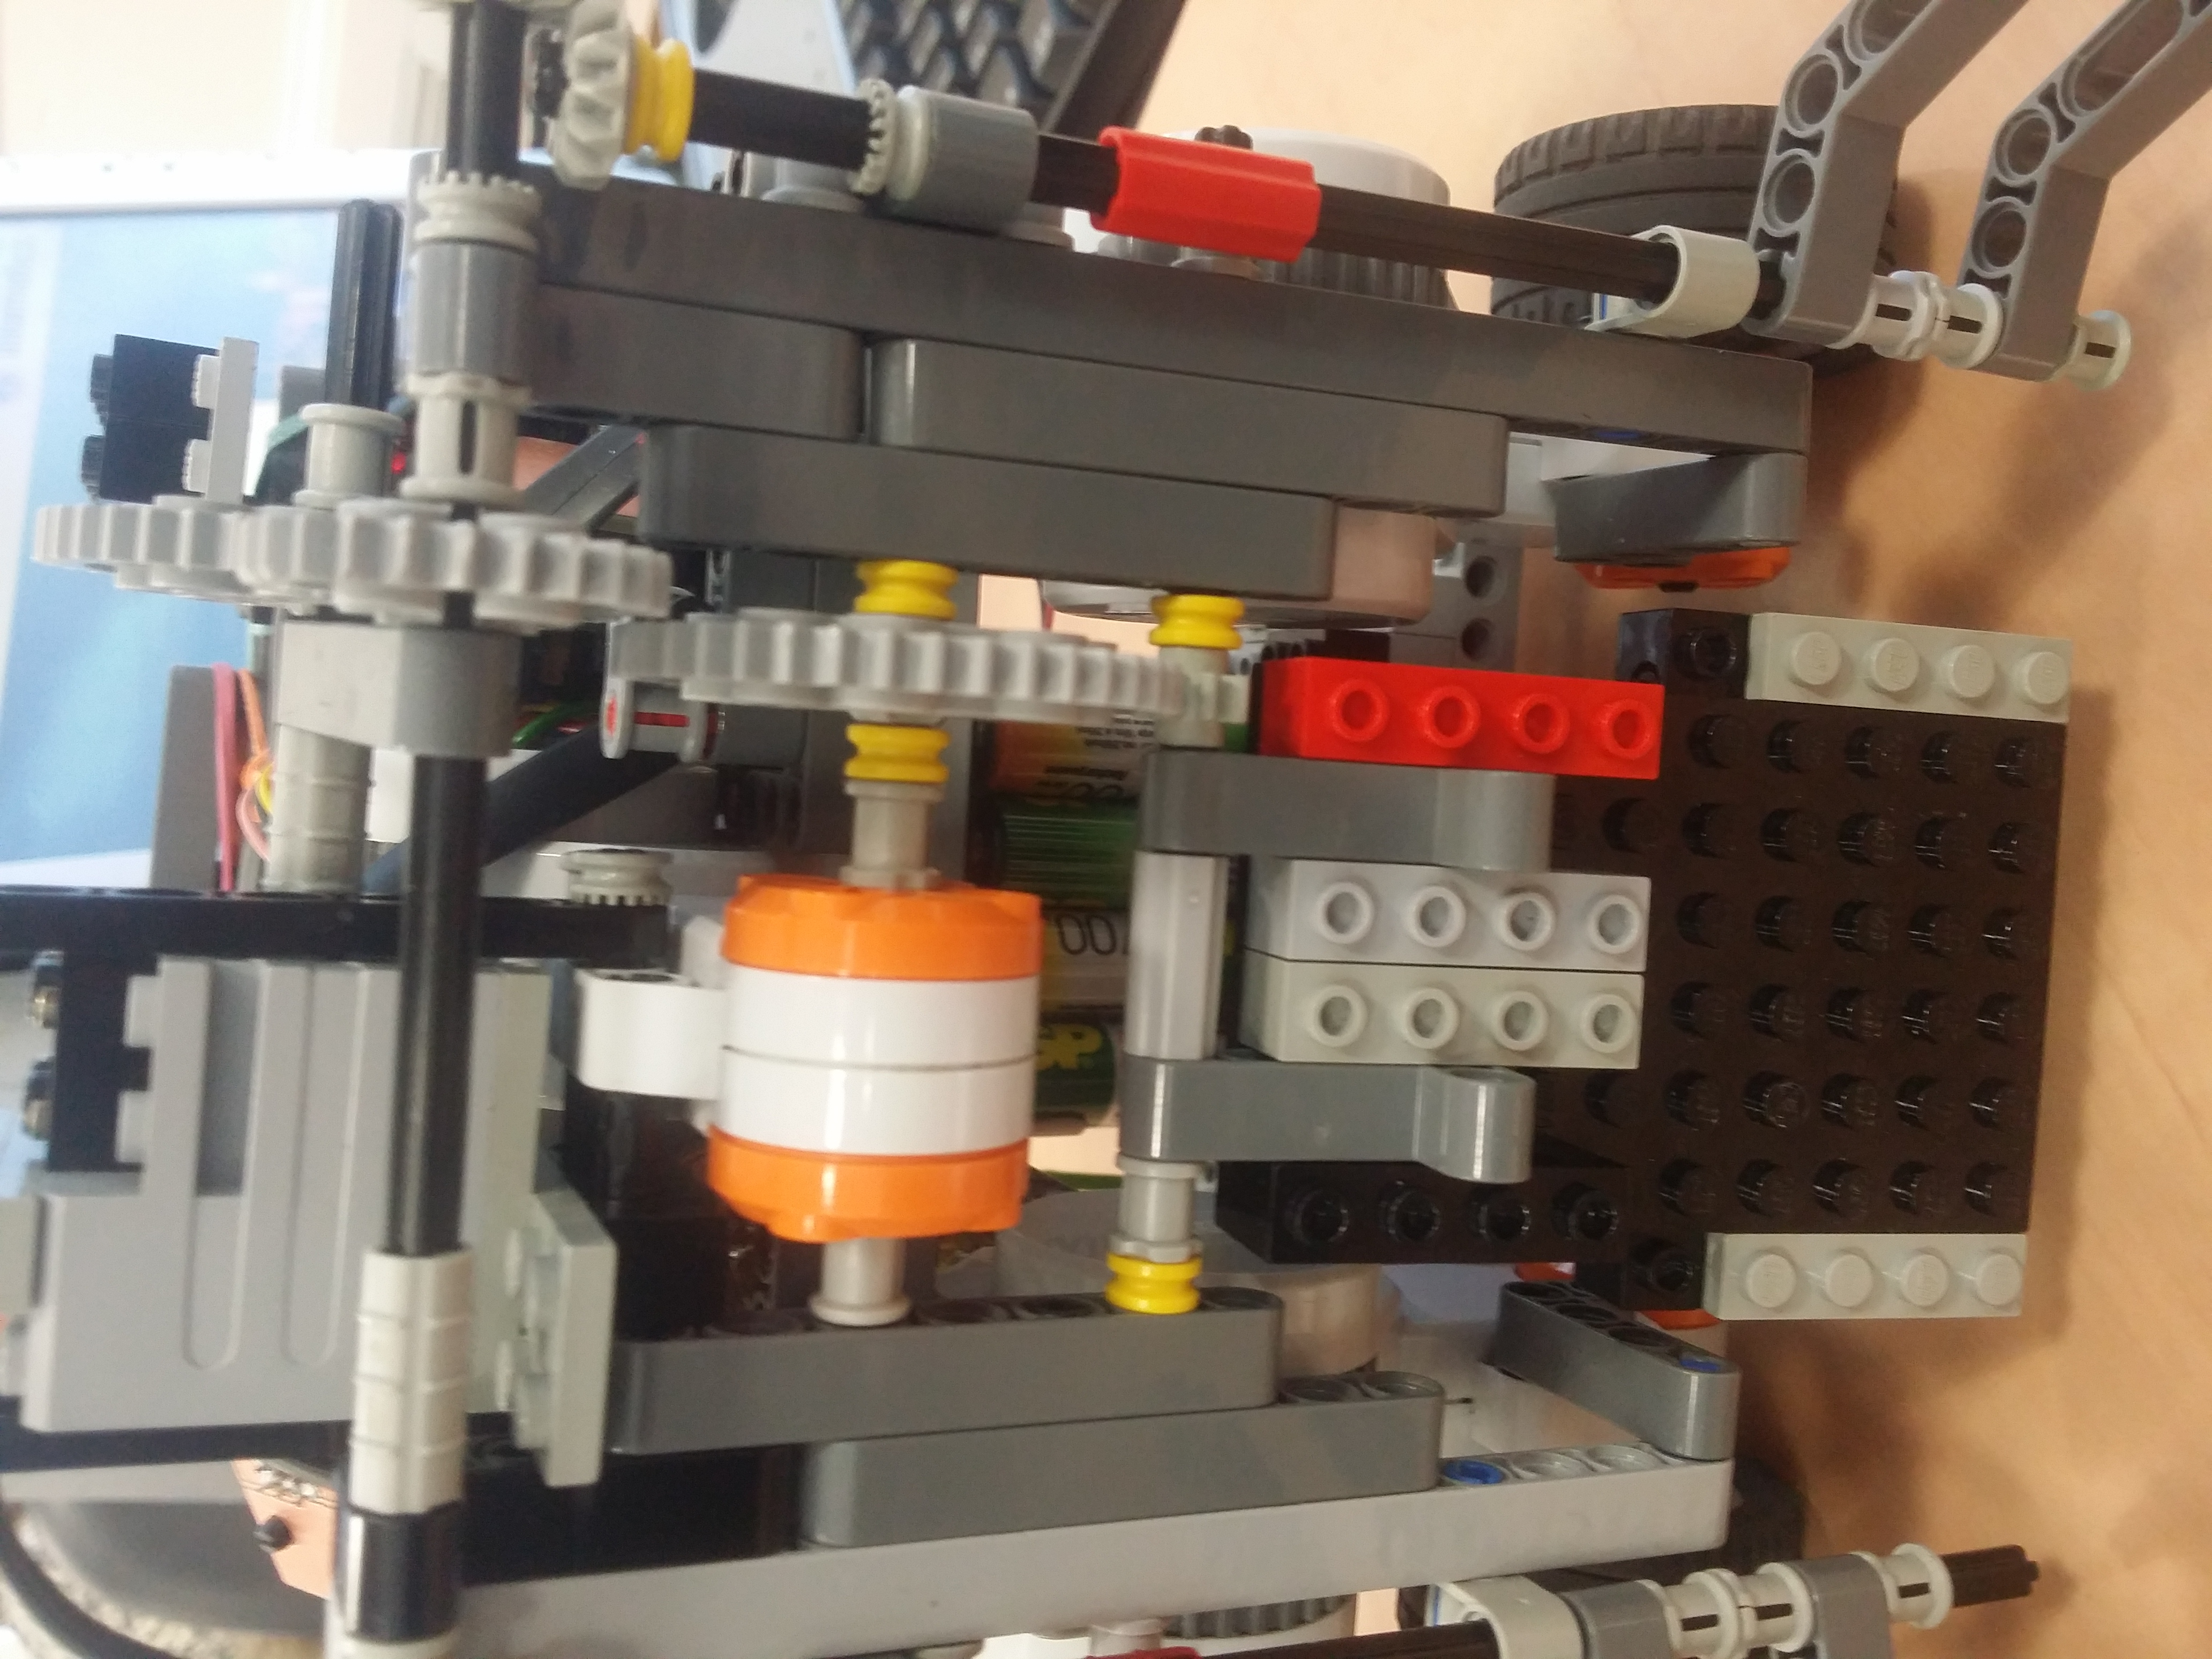
\includegraphics[scale=0.04, angle=-90]{kick_front.jpg}
		\caption{Kicker in still position}
		\label{fig:kicker}
	\end{minipage}
	~
	\begin{minipage}[b]{.3\textwidth}
        \centering
		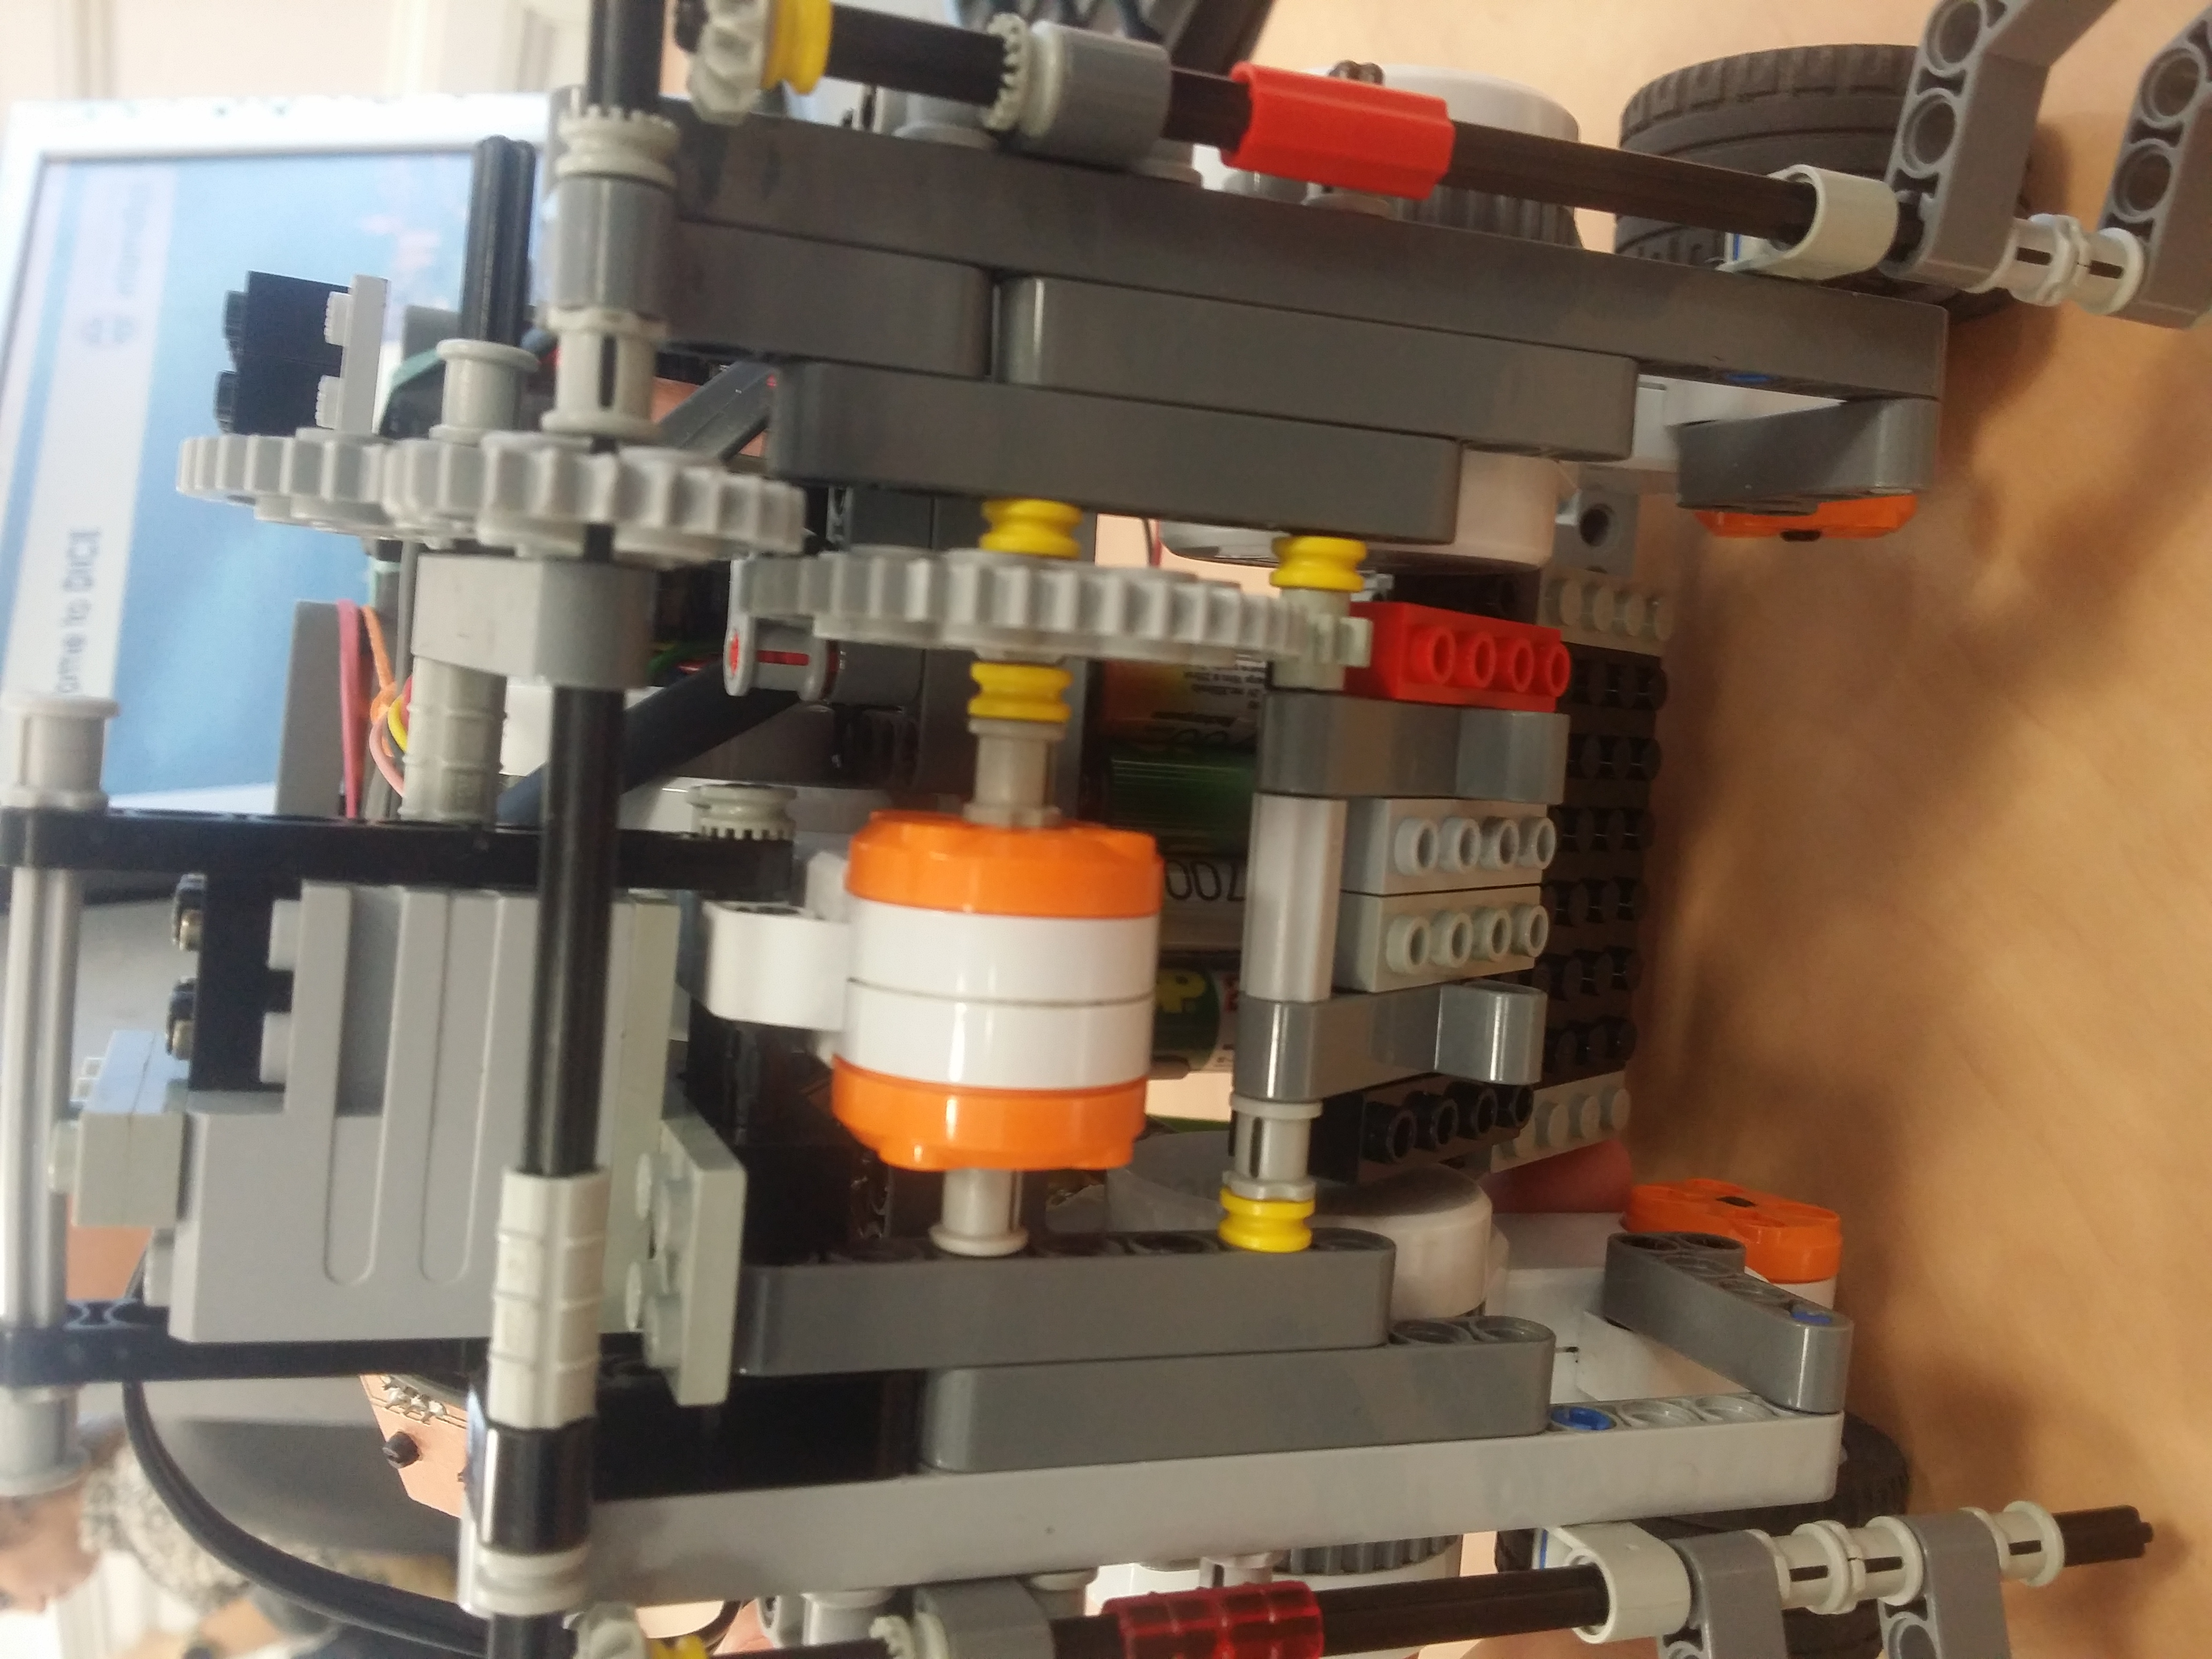
\includegraphics[scale=0.04, angle=-90]{kick_middle.jpg}
		\caption{Kicker starts going back}
		
	\end{minipage}
	~
	\begin{minipage}[b]{.3\textwidth}
        \centering
		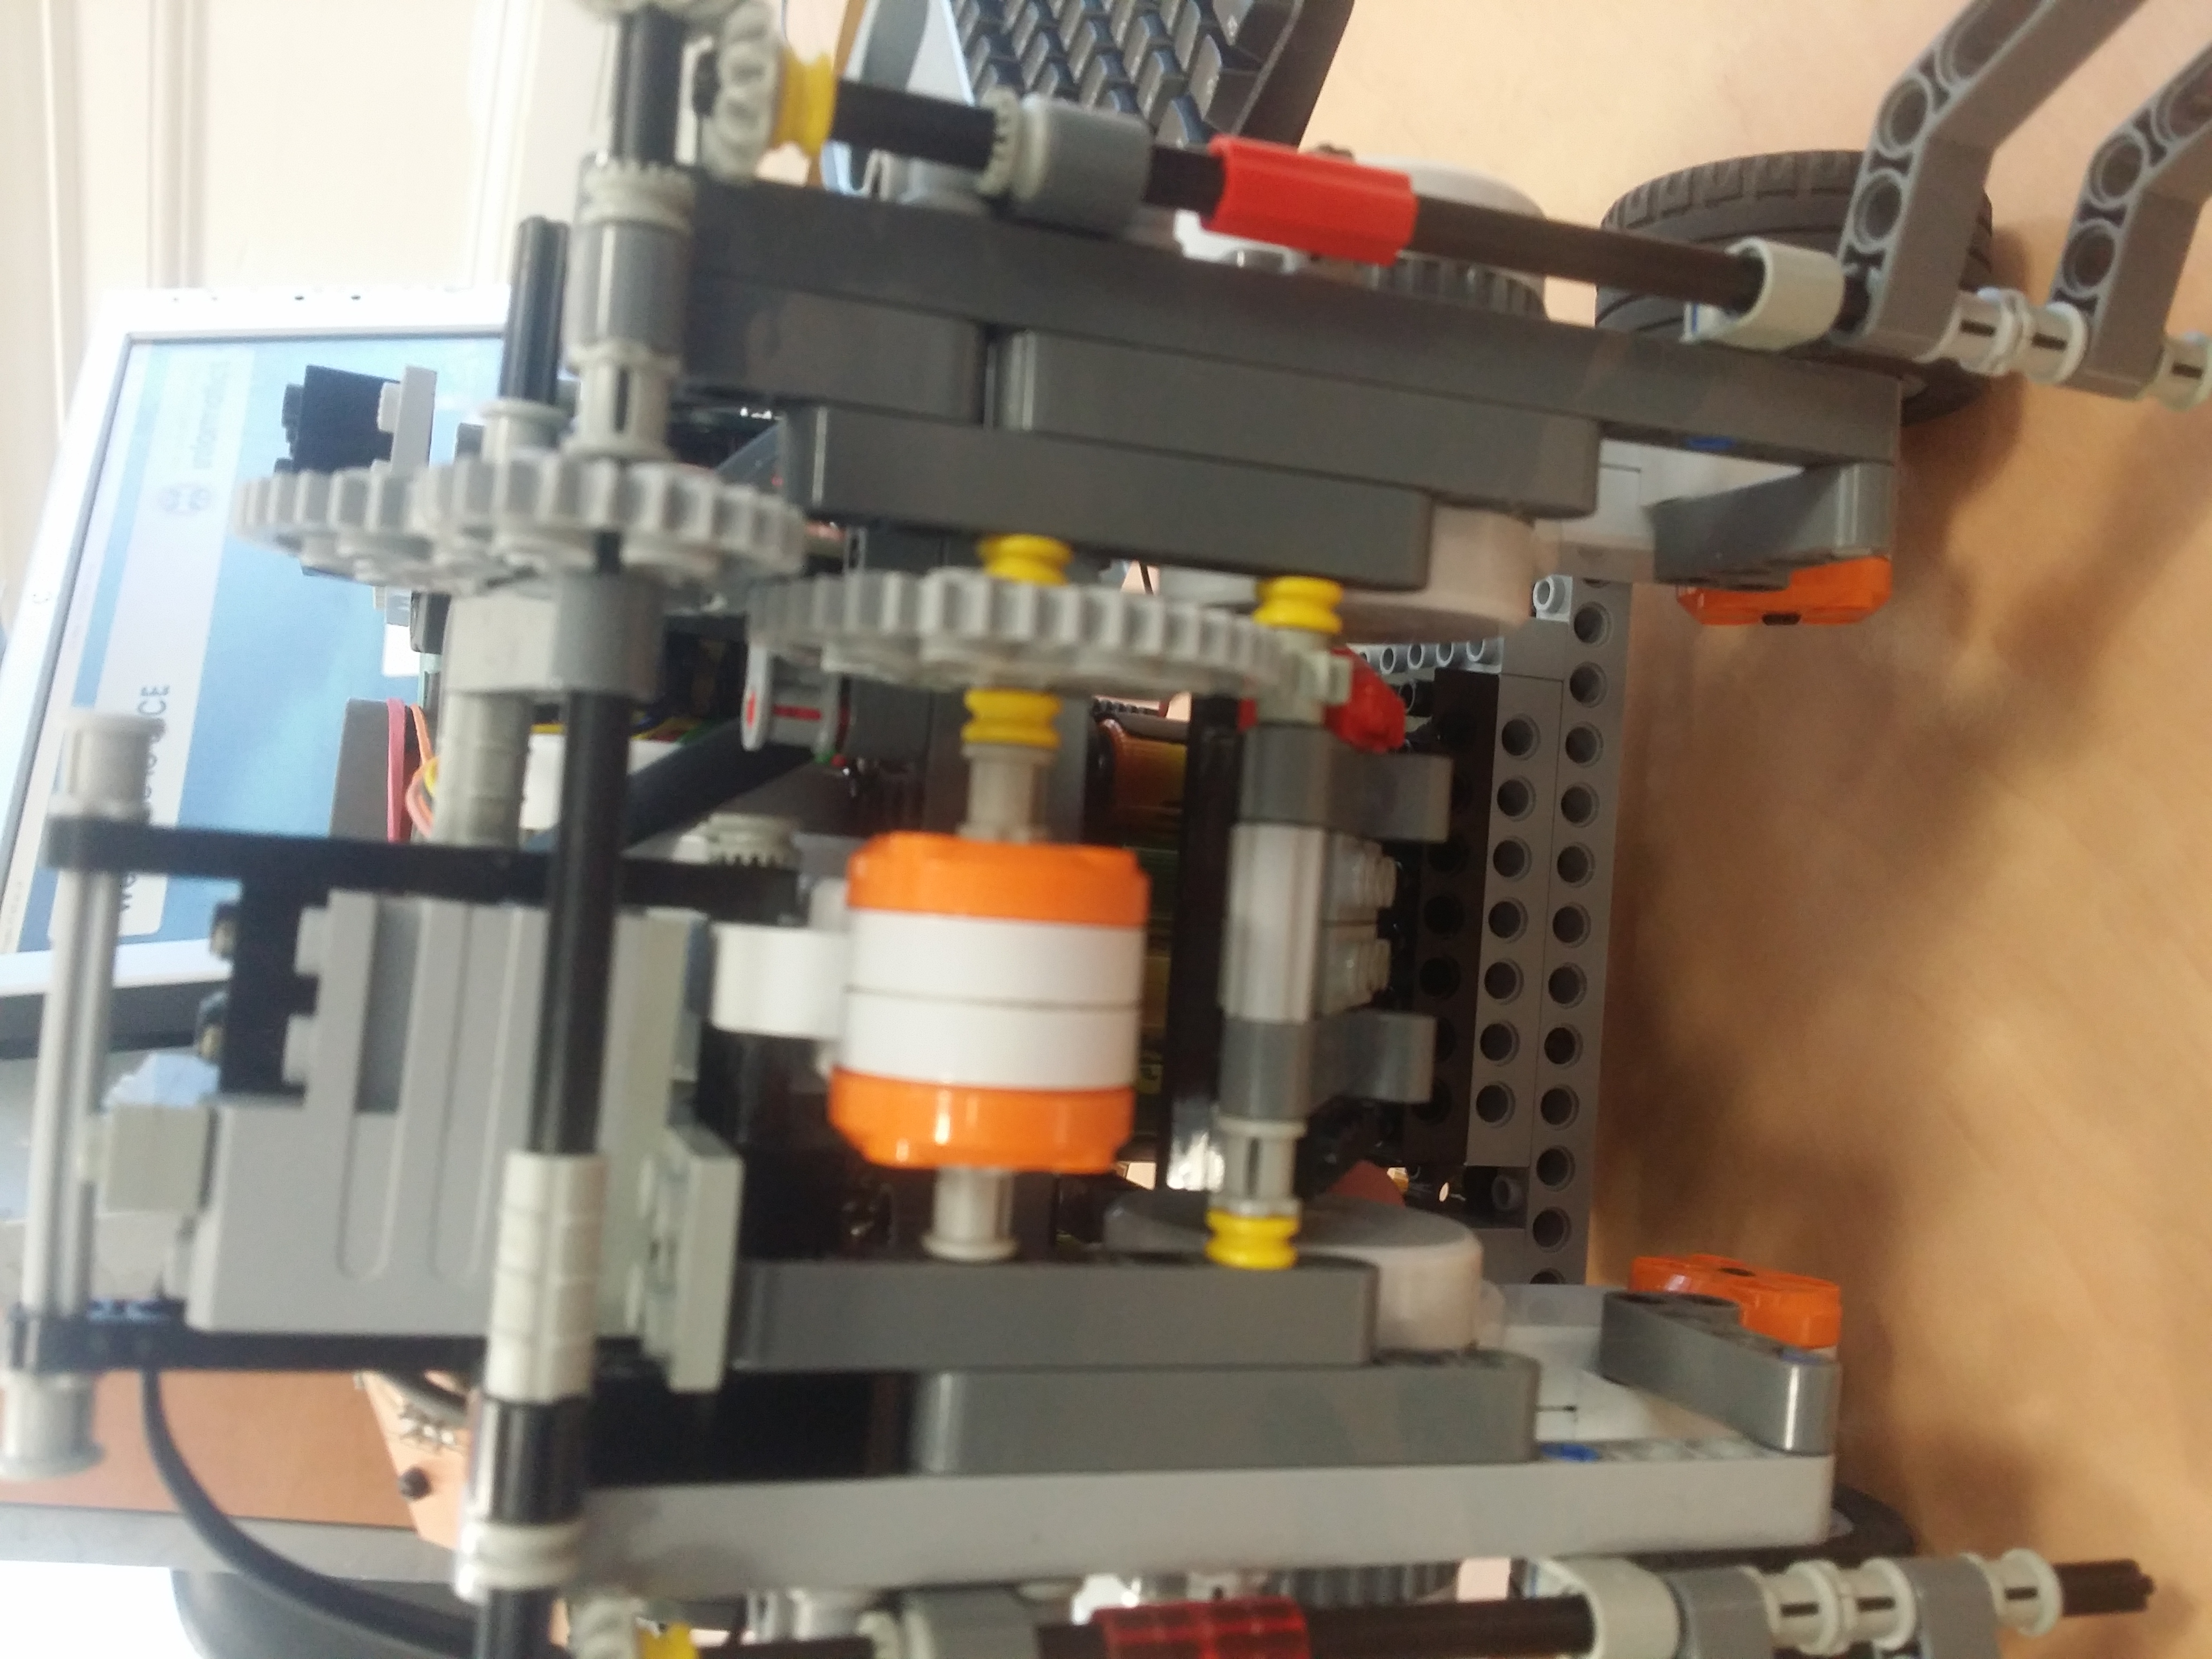
\includegraphics[scale=0.04, angle=-90]{kick_back.jpg}
		\caption{Kicker in the back position}
		\label{fig:kicker_back}
	\end{minipage}
	
\end{figure}

Our newest design doesn't have a kicker. The kick is made by turning  the robot and opening the grabber at the same time. This creates a momentum necessary to make a kick (Figure \ref{fig:kick_action}). 
\begin{figure}
    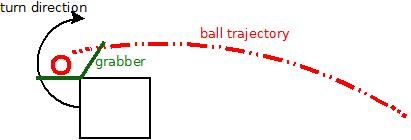
\includegraphics[scale=.7]{kick}
    \caption{High level diagram of how the kick is performed}
    \label{fig:kick_action}
\end{figure}


\subsection{Grabber}
The grabber for the previous design consisted of two symmetric parts placed one a bit above the other and was placed on the sides of the front part of the robot (Figure \ref{fig:gears}). They interlocked when the robot needs to catch the ball and we also kept them in a closed position during movements without the ball. We opened the grabber only before catching. This ensured that the grabber don't get broken against other robots or walls. We have used two bevel gears in order to be able to move grabbers with motor being on top of the robot. The current design of the grabber doesn't differ much and can be seen in Figure FIGURE. The grabber is powered by a single Electric Technic Mini-Motor 9v with gears.

\section{Documentation of the code}

\subsection{Communications}

The communication interface between the Arduino and PC is low level, that is,
the PC decides and specifies the individual motor numbers and rotary encoder
values or time durations for which they are going to be powered. Then the robot
turns the motors on, sets the timeouts to stop them, and notifies the PC about
finishing starting the motors.
\\The messages are human-readable, newline-terminated and tokens inside them are
separated by spaces. The following messages are available:

\begin{tabular}{ | l | l | }
    \hline
    Rotate the motors for $n$ ms &
    \texttt{M <n> <motorCount> <no> <power>...} \\ \hline
    Rotate the motors until $n$ rotary value &
    \texttt{R <n> <motorCount> <no> <power>...} \\ \hline
    Stop all motors &
    \texttt{S} \\ \hline
    Transfer a byte to I2C bus &
    \texttt{T <byteInDecimalASCII>} \\ \hline
\end{tabular}

The specified motor power can be negative, in which case it means backwards
direction.

\subsection{Arduino}

Arduino code uses \textit{SDPArduino} library to interact with the motors.
It also uses \textit{SerialCommand} library to buffer and tokenize the
commands received over the serial link. As seen before, there are two methods to
specify when to stop the motor: either time value or rotary encoder value.
In the case of time value a timeout is set to stop each single motor using
\textit{setTimeout} from the \textit{SimpleTimer} library.
In the case of rotary encoder value \textit{setInterval} is used which calls
a callback that queries the rotary encoder board each 30 ms and stops the motors
that reached the target rotary encoder value. These approaches using timers
allows the robot to receive commands asynchronously, that is, a command is not
blocking during its execution and the PC software could, for example, decide
to engage the kicker while the robot is in motion.

\subsection{PC}

The PC currently provides a simple command line interface. We use commands specified in the user guide such as \texttt{f 100} meaning 'go forwards 100 meters' that are mapped to communication messages, in our python code. We then are able to run this code from the command line.  

\subsection{Vision}

In our opinion, the vision is our unique feature of this project. We have built the whole system from scratch without borrowing any code from previous years. This allowed us to implement things we might not have been able to do with an existing system. 
\\In order to be able to detect robots and the ball, we go through the following steps:

\begin{enumerate}
\item For the relevant room (0 or 1) read files containing the following data: brightness, contrast,     saturation, hue values (room0.txt), minimum and maximum HSV values for each color that we want to detect (color0.txt), distortion (dist0.txt). 
\item The image from the video feed is blurred (using \textit{cv2.GaussianBlur}) and the mask is created (there is a possibility of calibration if some colors are not detected well enough).
\item We draw circles of relevant colors that are in the mask except red (the ball).
\item Find the ball.
\item Find robots.
\end{enumerate}

\subsubsection{Calibration}
When the video feed is opened, there are bars on the top that allow you to adjust brightness, hue, saturation and contrast. There is also a bar that is called 'calibration', which takes boolean values 0 or 
1. If you want to calibrate, you just need to move this bar to the right. 
\\When calibration mode is chosen another frame is opened, (it is a picture of the pitch captured when you entered this mode). In the top left corner, there is a ball representing the color that is currently being calibrated. In order to calibrate, you need to click on the pixels of this color. If the values that are read when you click do not match those expected for this color, they are discarded. With each new click a HSV values are stored, when calibration is finished, the range of all clicks is calculated for each color. This means you need to click multiple times in order to get a better result. This range is then stored to a file color0.txt overwriting anything else that was there before. We have minimum and maximum values for all colors except red, which has four values, because of the HSV cone. 
\\If you want to switch color, press 'q'. After all colors are done, the calibration mode is exited automatically. 

\subsubsection{Finding the robots}
Once we have detected all the colors, we try to decide where the actual robots are. In order to do that we need all robots to be on the pitch in the beginning when we run the code. 
\\There is a list of four robots we need to detect. We sort all colors we detected by their size (from biggest to lowest). Then for each robot, we check the following:

\begin{enumerate}
\item If we see all the colors on approximately right distances (given in rules) from each other, it is a perfect case and we say we have detected the robot.
\item If we can see the centre and the spot that is in bottom left corner (the one that differs from others), then we know the centre of mass, and we draw an orientation vector by rotating the line between centre and the spot we detected.
\item If we only can detect a centre spot, then we draw an orientation vector that we have seen in previous frame.
\item If there are three spots of the same color, then the centre of mass is calculated by taking the centre of two furthest from each other points. It is not exact, but gives a good approximation. The orientation vector is then drawed through the centre of mass and the middle point of two front spots.
\end{enumerate}
This ensures that we are able to detect robots even if at some point we cannot detect all the colors. Apart from the above steps, we also check that the centre of mass is on the reasonable distance from where it was in the last frame (to avoid robots flipping). Furthermore, if we have found the robot of one type (say our teammate), then we restrict it from finding another one. 
\\When the robots are found we draw a box around them (green for Venus and yellow for teammate red for opposite team) and label with a number from 0 to 3, where 0 is Venus, 1 is our teammate and 3,4 are opposite team robots. 

\subsubsection{Finding the ball}

We restrict the number of circles of each color we want to detect, e.g. 2 blue, 2 yellow, 8 green etc. For red, it is 9, because we are likely to think that pink is red. If at any point we are not able to see any red spots, we decide that the ball is underneath one of the robots or not on the pitch. If we can see the spot that is not part of the robots detected earlier, we store ball's position as a stack that has centres of mass of the ball for the last 6 frames (every time new value comes in, last one is popped). We check the first and the last values in this stack. If their difference is more than 10 pixels, then the ball is moving and we draw its trajectory.  

\subsection{Planning}

TBD

\subsection{Strategy}

The high-level overview of the system structure can be found in Figure \ref{fig:strategy}. It is not fully implemented yet.
\begin{figure}
    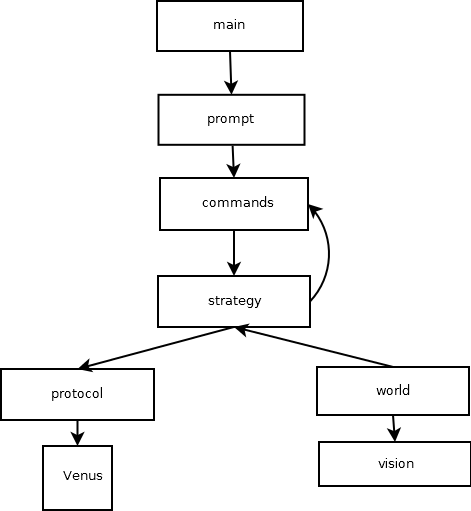
\includegraphics[scale=.7]{Diagram2}
    \caption{High level diagram of the system structure}
    \label{fig:strategy}
\end{figure}

\section{Sensors}
\subsection{Rotary encoder board}

Each NXT motor is connected to the rotary encoder board. This way the
information about how many rotations the motor performed since the last query
is available for the Arduino code. Every 30 ms we query the board and
check whether we have reached the target value. After the rotary value becomes
greater or equal to the target value, the appropriate motor is stopped.

\subsection{IR sensor}

TBD
\end{document}
